\documentclass{article}
\usepackage{microtype,graphicx,booktabs,hyperref,amsmath,amssymb}
\newcommand{\theHalgorithm}{\arabic{algorithm}}
\usepackage[preprint]{icml2026}
\icmltitlerunning{Frozen Scheduling in a Native Mechanical Robot Fixture}
\makeatletter\gdef\icmlcorrespondingauthor@text{Author details pending}\makeatother
% Generated only after final root all16 report gate; no worker outcome access.
\newcommand{\ReportMode}{FINAL AUDITED MECHANICAL SIMULATION COMPONENT}
\newcommand{\ResultAbstract}{All sixteen satisfy mechanical prerequisites. Primary T/F/U is 8/2/6; UNKNOWN is not a definite physical violation. Calibrated midpoint and exact joint grid each certify four of four timing tests, but strict hold and primary-plus-hold are zero of sixteen. These paired results establish no exact-grid or learned-policy advantage.}
\newcommand{\MethodRows}{Nominal & 0/2/2 & 4/4 & 0/4 & 0/4 \\
FIFO prior & 0/0/4 & 4/4 & 0/4 & 0/4 \\
Cal. midpoint & 4/0/0 & 4/4 & 0/4 & 0/4 \\
Exact joint & 4/0/0 & 4/4 & 0/4 & 0/4 \\
}
\newcommand{\CaseRows}{m0.9/d0 & U & U & T & T \\
m0.9/d12 & F & U & T & T \\
m1.1/d0 & U & U & T & T \\
m1.1/d12 & F & U & T & T \\
}
\newcommand{\ResultDiscussion}{Calibrated midpoint and exact joint grid have equal primary counts on these four fixed instances; this matrix does not establish an additional physical benefit from exact optimization. Both prior arms have eight INDETERMINATE contact intervals and eight INDETERMINATE gap intervals combined; only two release intervals are LATE. Their zero certified-primary counts are not evidence of large physical lateness. A prior gap upper bound is about 25.00094 ms against frozen 25 ms: timestamp intervals crossing the boundary remain UNKNOWN; no post hoc tolerance or idealized tick replacement is allowed.}
\newcommand{\SampleCounts}{Test/calibration task samples: 224,132/53,732; RGBD snapshots: 816/36. Test/calibration allocated GPU-wall upper bounds: 1.171/0.301 h. Snapshots and fixed video frames do not add episodes or native steps.}
\newcommand{\IntervalCoverage}{Observed contact/release intervals are contained in the empirical calibration box in 16/16 and 16/16 tests. This is not a support or statistical coverage guarantee.}
\newcommand{\SourceShort}{0c3cff79}
\newcommand{\CalibrationShort}{0bfe857c}
\newcommand{\ReportInputSHA}{39fc19002c08adc7}

\begin{document}
\twocolumn[
\icmltitle{Frozen Same-Information Scheduling in a Native Mechanical Robot Fixture}
\begin{icmlauthorlist}\icmlauthor{Research development draft}{draft}\end{icmlauthorlist}
\icmlaffiliation{draft}{Mechanical simulation supplement; chemical and learning validation remain open}
\vskip .3in]
\printAffiliationsAndNotice{}
\begin{abstract}
\textbf{\ReportMode.} We compare four rule schedulers on sixteen
declared native IsaacLab/PhysX mechanical simulation episodes, four
fixed instances per rule, after four separate calibration episodes.
The original mechanical task, three physical-event timing terms,
strict sampled bilateral hold and their conjunction are scored
separately. These are prescribed robot skills and calibrated scheduling,
not a VLA, weight learning or chemical-endpoint experiment.
\ResultAbstract
\end{abstract}

\begin{table}[!ht]
\centering\small
\caption{All sixteen declared tests. Each method denominator is four.
Primary, mechanical task, strict sampled hold and primary+hold are
different predicates. All entries use the complete frozen roster.}
\begin{tabular}{lrrrr}\toprule
Rule & T/F/U & Mech. & Hold & Joint+H\\\midrule
\MethodRows\bottomrule
\end{tabular}
\end{table}

\begin{figure*}[t]
\centering
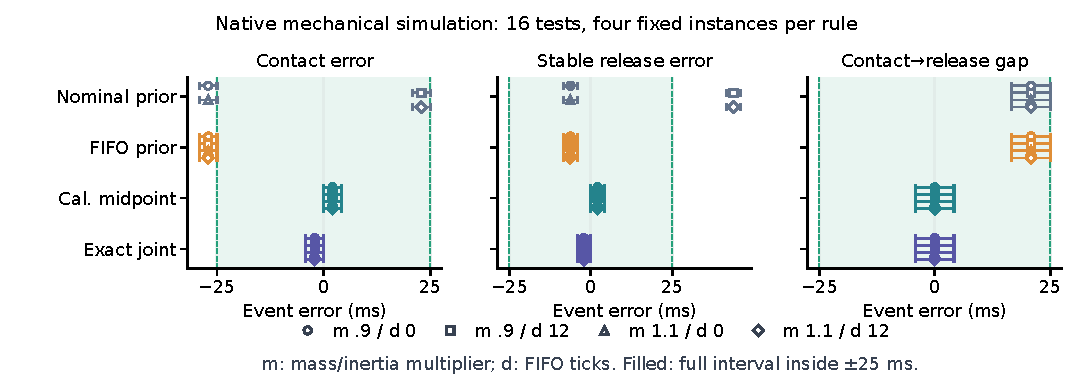
\includegraphics[width=\textwidth]{../generated/robot_timing_intervals_paper.pdf}
\caption{All sixteen tests, three event terms, frozen $\pm25$ ms region.
Final markers and error bars come only from the root's complete audited
report. A timing pass does not imply strict hold. Mechanical simulation,
not RGB, hardware, chemical outcome or VLA evidence.}
\end{figure*}

\begin{table*}[t]
\centering\small
\caption{Complete primary T/F/U matrix: four conditions by four rules, all sixteen tests. U is unknown, not a definite violation. m is a dimensionless mass/inertia multiplier; d is FIFO ticks. Full case ids, hold and timing intervals remain in the all-sixteen CSV.}
\begin{tabular}{lcccc}\toprule
Condition & Nominal & FIFO & Midpoint & Exact\\\midrule
\CaseRows\bottomrule
\end{tabular}
\end{table*}
\section{Frozen experiment and causal scope}
The fixed mechanical component uses the original bottle-operation
skill with a prospectively qualified hand stiffness of 1600, preserved
mechanical criteria and frozen $\pm25$ ms timing contracts. Only
position-target hold timing is varied; physical state and time are not
overwritten. Four new calibration instances use dimensionless mass/inertia factors .8/1.2
and FIFO delays 0/12 ticks. Their frozen empirical min/max ranges are
not certified model support. Four test instances use .9/1.1 dimensionless factors and
the same two FIFO conditions: interpolation, not mass extrapolation.
Deadline values 5/5.5 s and duration values 18/18.5 s are tied to these
conditions, preventing independent mass/deadline/duration attribution.
Source \texttt{\SourceShort} and calibration \texttt{\CalibrationShort}
are bound before test execution.

All methods share public information, the skill and mechanical
controller. Nominal prior and public FIFO correction provide uncalibrated comparators; calibrated midpoint and exact joint grid
use the same four-instance calibration. No test outcome adjusts the
gains, tolerance, priors or scheduling formulas. Native stepping is
240 Hz. FIFO delays position targets, while gravity compensation and
guards remain immediate; this is not whole-communication or actual
LLM-inference latency. Host execution cost is reported separately. These frozen bottle-task
targets do not demonstrate recovery against an independently observed
irreversible external chemical event.

\section{Independent physical semantics and denominator}
Bilateral contact onset requires the declared contact window;
confirmation is recorded separately. Release is the onset of the
original supported, unloaded, open-jaw, upright, stable eight-sample
window, not first unloading. The elapsed contact-to-release term is a
timing relation, not proof of continuous holding. For occurrence
intervals $[\ell_a,u_a]$ and $[\ell_b,u_b]$, timing error is
\[
 [\ell_b-u_a-D,\ u_b-\ell_a-D].
\]
Only full containment in the frozen window passes. Partial overlap,
missing endpoints and refusal cannot become success. Every declared
episode stays in the sixteen-test denominator; the four calibration
episodes remain separate. Primary requires all three timing terms
and the original mechanism. Strict hold checks every sampled point
under its original definition; negative post-opening/pre-release
points remain. Their conjunction is reported in the same front table.



\section{Evidence and attribution limits}
\ResultDiscussion\ \IntervalCoverage\ \SampleCounts\par
Four deterministic scene conditions provide paired mechanism
evidence, not random-seed statistics, confidence intervals or unseen
task-space generalization. Full numeric nine-joint K/D/effort arrays
are read at before/after/end snapshots, not continuously per tick.
Fresh and cached physical-state preimages are independently checked.
Equality at three endpoints cannot establish hidden solver-state or
between-snapshot parameter invariance. There are zero new policy
weight updates, real-robot episodes and independent chemical endpoints.

An explicit historical correction is retained: all four old
calibration traces exported actual K/D/effort arrays at the 1200-step
warmup endpoint. The earlier claim of no active readbacks was too
broad, including the frozen metadata literal. They still lack the
new dedicated after-30 and before/after/end full snapshots; saved
comparison flags do not restore numeric arrays. Original sources,
scores, failed admissions, budgets and denominators are unchanged.
See \href{../../../independent_audit/LEGACY_ACTIVE_READBACK_CORRECTION.json}
{LEGACY\_ACTIVE\_READBACK\_CORRECTION.json} and its Chinese note.

\paragraph{Report binding.}
Generated numerical content must bind the complete root report,
all-sixteen CSV and vector plot, source/calibration hashes and the
legacy correction. Report SHA prefix: \texttt{\ReportInputSHA}.
This supplement does not establish a new learned algorithm.
\end{document}
